\documentclass[11pt,a4paper]{article}

\usepackage[a4paper,margin=1in]{geometry}
\usepackage{amsmath}
\usepackage{amssymb}
\usepackage{booktabs}
\usepackage{array}
\usepackage{longtable}
\usepackage{graphicx}
\usepackage{float}
\usepackage{placeins}
\usepackage{graphicx}
\usepackage{float}
\usepackage{placeins}
\usepackage{hyperref}
\usepackage{enumitem}
\usepackage{hyperref}
\usepackage{enumitem}
\usepackage{titlesec}
\usepackage{listings}
\usepackage{xcolor}

\hypersetup{
colorlinks=true,
linkcolor=blue,
urlcolor=blue
}

\lstset{
language=Python,
basicstyle=\ttfamily\small,
keywordstyle=\color{blue},
commentstyle=\color{green!50!black},
stringstyle=\color{red},
numbers=left,
numberstyle=\tiny,
stepnumber=1,
breaklines=true,
frame=single,
showstringspaces=false
}

\renewcommand{\arraystretch}{1.4}

\begin{document}
\raggedbottom

\setlength{\textfloatsep}{10pt}
\setlength{\floatsep}{8pt}
\setlength{\intextsep}{8pt}

\clubpenalty=10000
\widowpenalty=10000
\displaywidowpenalty=10000

\begin{center}

{\Large \textbf{Shiv Nadar University Chennai}}

\vspace{0.3cm}

\begin{tabular}{|p{4cm}|p{8cm}|p{2cm}|}
\hline
Degree \& Branch &
B.Tech Artificial Intelligence \& Data Science &
Semester V\\
\hline
Subject Code \& Name &
CS3807 -- Deep Learning Laboratory &
AY: 2026--27\\
\hline
\end{tabular}

\vspace{0.7cm}

{\Large \textbf{Experiment 1}}

\vspace{0.2cm}

{\large \textbf{Implementation of a Single Layer Perceptron for Binary Classification}}

\end{center}

\section*{1. Objective}

The objective of this experiment is to understand the working principle of an Artificial Neuron and implement a Single Layer Perceptron from scratch for binary classification. The Banknote Authentication dataset is used to train and evaluate the perceptron model. The experiment also aims to study the effect of feature normalization, analyse the learning behaviour using different plots and evaluate the classifier using standard performance metrics such as Accuracy, Precision, Recall and F1-score.

\section*{2. Background Theory}

Artificial Neural Networks are computational models inspired by the functioning of biological neurons. The fundamental processing unit of an Artificial Neural Network is the Artificial Neuron. Each neuron receives several input features, multiplies them with trainable weights, adds a bias value and passes the result through an activation function to generate an output.

The Single Layer Perceptron proposed by Frank Rosenblatt is one of the earliest supervised learning algorithms. It is capable of solving only linearly separable binary classification problems. During training, the perceptron iteratively updates its weights and bias using the perceptron learning rule until the classification error is minimized.

\subsection*{Mathematical Formulation}

The weighted sum of the inputs is

\[
z=\mathbf{w}^{T}\mathbf{x}+b
\]

where

\begin{itemize}
\item $\mathbf{x}$ denotes the input feature vector.
\item $\mathbf{w}$ denotes the weight vector.
\item $b$ denotes the bias.
\item $z$ denotes the weighted sum.
\end{itemize}

The output of the perceptron is

\[
\hat{y}=f(z)
\]

where $f(z)$ represents the activation function.

The perceptron learning rule updates the weights according to

\[
\mathbf{w}_{new}
=
\mathbf{w}_{old}
+
\eta
(y-\hat{y})
\mathbf{x}
\]

The bias is updated using

\[
b_{new}
=
b_{old}
+
\eta
(y-\hat{y})
\]

where

\begin{itemize}
\item $\eta$ is the learning rate.
\item $y$ is the actual class.
\item $\hat{y}$ is the predicted class.
\end{itemize}
\section*{3. Activation Function}

An activation function determines the output of a neuron based on its weighted input. In this experiment, the Step Activation Function is employed because the problem involves binary classification. The function produces either 0 or 1 depending on the value of the weighted sum.

\[
f(z)=
\begin{cases}
1,&z\ge0\\
0,&z<0
\end{cases}
\]

The Step Activation Function is simple and computationally efficient. However, it is not differentiable and therefore cannot be used with gradient-based optimization algorithms such as backpropagation.

\vspace{0.15cm}

\begin{center}
\begin{tabular}{|c|c|p{7cm}|}
\hline
\textbf{Activation Function} & \textbf{Output Range} & \textbf{Typical Application}\\
\hline
Step & $\{0,1\}$ & Classical Perceptron\\
\hline
Sigmoid & $(0,1)$ & Binary Classification Output Layer\\
\hline
Tanh & $(-1,1)$ & Hidden Layers\\
\hline
ReLU & $[0,\infty)$ & Deep Neural Networks\\
\hline
Leaky ReLU & $(-\infty,\infty)$ & Avoiding Dying ReLU\\
\hline
Softmax & $(0,1)$ & Multi-class Classification\\
\hline
\end{tabular}
\end{center}

\vspace{0.3cm}

Although several activation functions exist, only the Step Activation Function is used in this experiment because the Single Layer Perceptron performs binary classification on linearly separable data.

 

\section*{4. Dataset Description}

The experiment uses the \textbf{Banknote Authentication Dataset} obtained from the UCI Machine Learning Repository. The dataset consists of statistical features extracted from digital images of genuine and forged banknotes using wavelet transforms.

\vspace{0.3cm}

\begin{center}
\begin{tabular}{|p{5cm}|p{7cm}|}
\hline
\textbf{Property} & \textbf{Value}\\
\hline
Dataset Name & Banknote Authentication Dataset\\
\hline
Source & UCI Machine Learning Repository\\
\hline
Total Samples & 1372\\
\hline
Input Features & 4\\
\hline
Target Classes & 2\\
\hline
Missing Values & None\\
\hline
Learning Type & Supervised Learning\\
\hline
Problem Type & Binary Classification\\
\hline
\end{tabular}
\end{center}

\vspace{0.15cm}

\textbf{Feature Description}

\begin{center}
\begin{tabular}{|c|p{10cm}|}
\hline
\textbf{Feature} & \textbf{Description}\\
\hline
Variance & Variance of the wavelet transformed image.\\
\hline
Skewness & Degree of asymmetry in the image distribution.\\
\hline
Curtosis & Sharpness or flatness of the probability distribution.\\
\hline
Entropy & Measure of randomness present in the image.\\
\hline
\end{tabular}
\end{center}

\vspace{0.3cm}

\textbf{Target Classes}

\begin{itemize}
\item Class 0 -- Authentic Banknote
\item Class 1 -- Forged Banknote
\end{itemize}

The dataset contains no missing values and is well suited for demonstrating the learning capability of a Single Layer Perceptron after feature normalization.
 

\section*{5. Experimental Procedure}

The experiment was carried out using Python in Google Colab. The implementation followed a systematic workflow beginning from dataset loading to model evaluation.

\subsection*{Task 1: Dataset Exploration}

The dataset was first imported into the notebook using the Pandas library. The first five samples, dataset dimensions, missing values and descriptive statistics were obtained.

\textbf{Output}

\begin{itemize}
\item Total Samples : 1372
\item Total Features : 4
\item Target Classes : 2
\item Missing Values : None
\end{itemize}

\vspace{0.3cm}

The descriptive statistics indicated that the dataset contains features with different numerical ranges. Therefore, feature normalization was performed before training the perceptron model.

%%%%%%%%%%%%%%%%%%%%%%%%%%%%%%%%%%%%%%%%%%%%%%%%%%%%%%%%%%%%

\subsection*{Task 2: Exploratory Data Analysis}

Exploratory Data Analysis (EDA) was carried out to understand the characteristics of the dataset before model training.

The following visualizations were generated.

\begin{itemize}
\item Feature Histograms
\item Correlation Heatmap
\item Scatter Plot
\item Box Plot
\end{itemize}

These visualizations helped in identifying feature distributions, relationships among variables and the presence of outliers.

%%%%%%%%%%%%%%%%%%%%%%%%%%%%%%%%%%%%%%%%%%%%%%%%%%%%%%%%%%%%

\subsection*{Task 3: Data Preprocessing}

Before training, the dataset was preprocessed using the following steps.

\begin{enumerate}
\item Selected the four numerical features as input variables.
\item Selected the class column as the target variable.
\item Normalized all feature values using Min-Max Scaling.
\item Split the dataset into training and testing subsets.
\item Used an 80:20 train-test ratio.
\end{enumerate}

\vspace{0.3cm}

The normalized dataset ensured that all features contributed equally during weight updates.

%%%%%%%%%%%%%%%%%%%%%%%%%%%%%%%%%%%%%%%%%%%%%%%%%%%%%%%%%%%%

\subsection*{Task 4: Perceptron Implementation}

A Single Layer Perceptron was implemented completely from scratch without using any machine learning libraries.

The implementation consisted of

\begin{itemize}
\item Weight Initialization
\item Bias Initialization
\item Step Activation Function
\item Forward Propagation
\item Perceptron Learning Rule
\item Weight Update
\item Bias Update
\end{itemize}

The weights were initialized with small random values and updated after every misclassified sample according to the perceptron learning rule.

%%%%%%%%%%%%%%%%%%%%%%%%%%%%%%%%%%%%%%%%%%%%%%%%%%%%%%%%%%%%

\subsection*{Task 5: Model Training}

The perceptron was trained for a maximum of 100 epochs.

During every epoch,

\begin{itemize}
\item Forward propagation was performed.
\item Misclassified samples were identified.
\item Weights were updated.
\item Bias was updated.
\item Training error was recorded.
\end{itemize}

Training continued until all epochs were completed while monitoring convergence through the number of misclassified samples.

%%%%%%%%%%%%%%%%%%%%%%%%%%%%%%%%%%%%%%%%%%%%%%%%%%%%%%%%%%%%

\subsection*{Task 6: Model Evaluation}

After training, the classifier was evaluated using

\begin{itemize}
\item Accuracy
\item Precision
\item Recall
\item F1-Score
\item Confusion Matrix
\end{itemize}

The evaluation metrics measured the effectiveness of the trained perceptron on unseen testing samples.

%%%%%%%%%%%%%%%%%%%%%%%%%%%%%%%%%%%%%%%%%%%%%%%%%%%%%%%%%%%%

 

\section*{6. Source Code}

The complete implementation was carried out in Python using Google Colab.
\\[10pt]
\url{https://github.com/K-Mithran/Deep-Learning/blob/main/Lab1/DL_1.ipynb}
\\[10pt]
The major stages of implementation included

\begin{enumerate}
\item Loading the dataset.
\item Performing exploratory data analysis.
\item Normalizing the dataset.
\item Splitting the dataset.
\item Implementing the perceptron from scratch.
\item Training the perceptron.
\item Evaluating the trained model.
\item Visualizing the learning behaviour.
\end{enumerate}

The complete source code used in this experiment is available in the submitted Google Colab notebook and GitHub repository.
 

\section*{7. Experimental Results}

\subsection*{7.1 Dataset Exploration}

The Banknote Authentication dataset was successfully loaded into Google Colab. The dataset contains four numerical input features and one binary target class.

\begin{center}
\begin{tabular}{|p{6cm}|p{5cm}|}
\hline
\textbf{Property} & \textbf{Observed Value}\\
\hline
Dataset Size & 1372 Samples\\
\hline
Number of Features & 4\\
\hline
Number of Classes & 2\\
\hline
Missing Values & 0\\
\hline
Training Samples & 1097\\
\hline
Testing Samples & 275\\
\hline
\end{tabular}
\end{center}

\vspace{0.15cm}

The dataset was found to be complete with no missing values. The descriptive statistics showed noticeable differences in feature ranges, making feature normalization necessary before training.

%%%%%%%%%%%%%%%%%%%%%%%%%%%%%%%%%%%%%%%%%%%%%%%%%%%%%%%%%%%%%%

\subsection*{7.2 Data Preprocessing Results}

After applying Min-Max Normalization, every feature value was transformed into the range [0,1].

The dataset was divided into

\begin{itemize}
\item Training Set : 80\%
\item Testing Set : 20\%
\end{itemize}

This preprocessing step improved convergence during perceptron training.

%%%%%%%%%%%%%%%%%%%%%%%%%%%%%%%%%%%%%%%%%%%%%%%%%%%%%%%%%%%%%%

\subsection*{7.3 Model Training}

The perceptron was trained for 100 epochs.

During training, the number of misclassified samples gradually reduced while the weights and bias converged to stable values.

The final learned parameters are shown below.

\vspace{0.15cm}

\begin{center}
\begin{tabular}{|p{6cm}|p{6cm}|}
\hline
\textbf{Parameter} & \textbf{Value}\\
\hline
Weight 1 & -0.2301\\
\hline
Weight 2 & -0.2384\\
\hline
Weight 3 & -0.2603\\
\hline
Weight 4 & 0.0007\\
\hline
Bias & 0.31\\
\hline
Maximum Epochs & 100\\
\hline
\end{tabular}
\end{center}

%%%%%%%%%%%%%%%%%%%%%%%%%%%%%%%%%%%%%%%%%%%%%%%%%%%%%%%%%%%%%%

\subsection*{7.4 Performance Metrics}

The trained perceptron was evaluated on the testing dataset using standard classification metrics.

\vspace{0.3cm}

\begin{center}
\begin{tabular}{|p{6cm}|c|}
\hline
\textbf{Metric} & \textbf{Value}\\
\hline
Accuracy & 98.18\%\\
\hline
Precision & 100.00\%\\
\hline
Recall & 96.03\%\\
\hline
F1-Score & 97.98\%\\
\hline
\end{tabular}
\end{center}

The obtained results indicate that the perceptron successfully classified the majority of unseen testing samples. The perfect precision value indicates that every banknote predicted as forged was indeed forged, while the high recall confirms that almost all forged banknotes were correctly identified.

%%%%%%%%%%%%%%%%%%%%%%%%%%%%%%%%%%%%%%%%%%%%%%%%%%%%%%%%%%%%%%

\subsection*{7.5 Learning Rate Comparison}

The perceptron model was trained using three different learning rates to study their influence on model performance.

\begin{center}
\begin{tabular}{|c|c|c|}
\hline
\textbf{Learning Rate} & \textbf{Epochs} & \textbf{Accuracy}\\
\hline
0.001 & 100 & 99.64\%\\
\hline
0.010 & 100 & 99.64\%\\
\hline
0.100 & 100 & 98.91\%\\
\hline
\end{tabular}
\end{center}

The comparison shows that learning rates of 0.001 and 0.01 achieved the highest classification accuracy. Increasing the learning rate to 0.1 resulted in a slight reduction in performance because of larger parameter updates during training.

%%%%%%%%%%%%%%%%%%%%%%%%%%%%%%%%%%%%%%%%%%%%%%%%%%%%%%%%%%%%%%

 

\section*{8. Performance Summary}

\begin{center}
\begin{tabular}{|p{7cm}|p{5cm}|}
\hline
Dataset Size & 1372\\
\hline
Training Samples & 1097\\
\hline
Testing Samples & 275\\
\hline
Features & 4\\
\hline
Learning Rate & 0.01\\
\hline
Epochs & 100\\
\hline
Final Bias & 0.31\\
\hline
Accuracy & 98.18\%\\
\hline
Precision & 100.00\%\\
\hline
Recall & 96.03\%\\
\hline
F1-Score & 97.98\%\\
\hline
\end{tabular}
\end{center}


\section*{9. Generated Plots with Interpretation}

%%%%%%%%%%%%%%%%%%%%%%%%%%%%%%%%%%%%%%%%%%%%%%%%%%%%%%%%%%%%%%

\subsection*{9.1 Feature Histograms}

\begin{figure}[H]
    \centering
    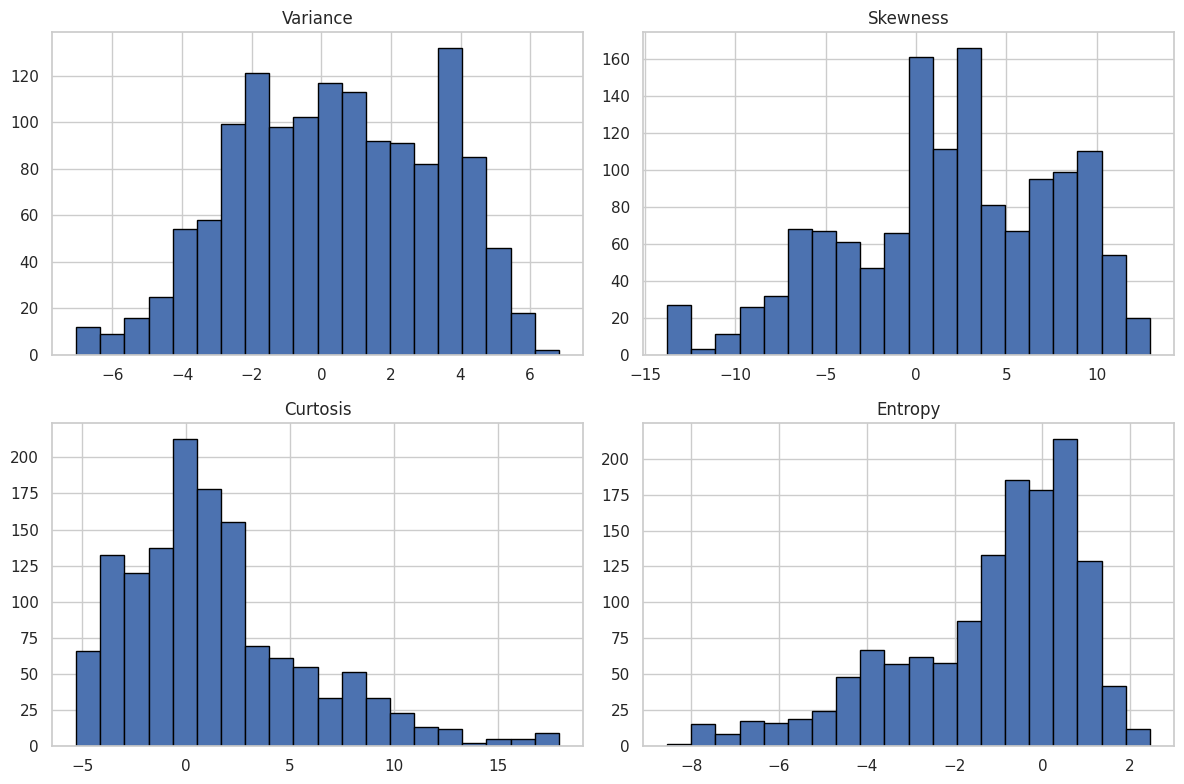
\includegraphics[width=0.90\textwidth]{histogram.png}
    \caption{Feature Histograms of the Banknote Authentication Dataset}
    \label{fig:histogram}
\end{figure}

The histograms illustrate the distribution of all four numerical features present in the dataset. The features exhibit different ranges and varying degrees of skewness, indicating that normalization is necessary before training the perceptron.

\vspace{0.3cm}

%%%%%%%%%%%%%%%%%%%%%%%%%%%%%%%%%%%%%%%%%%%%%%%%%%%%%%%%%%%%%%

\subsection*{9.2 Correlation Heatmap}

\begin{figure}[H]
    \centering
    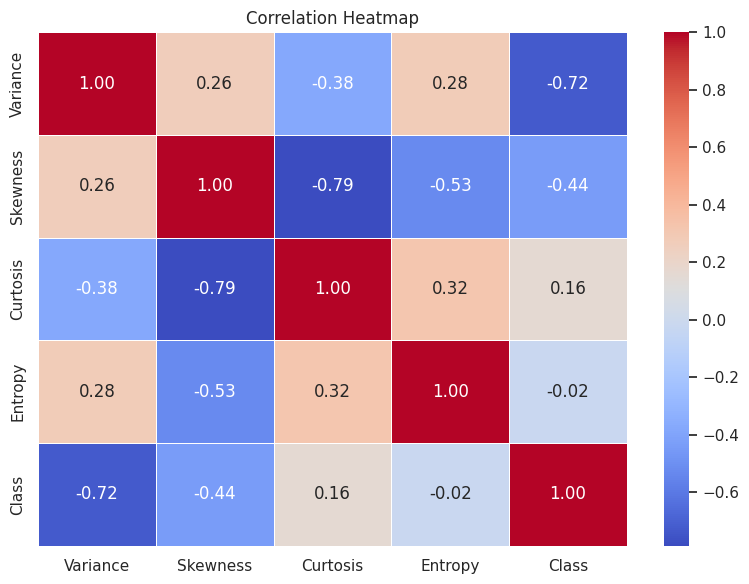
\includegraphics[width=0.66\textwidth]{heatmap.png}
    \caption{Correlation Heatmap}
    \label{fig:heatmap}
\end{figure}

The heatmap illustrates the correlation between the input features. Highly correlated features provide useful information regarding the relationships among variables and help in understanding the overall structure of the dataset.

\vspace{0.3cm}

%%%%%%%%%%%%%%%%%%%%%%%%%%%%%%%%%%%%%%%%%%%%%%%%%%%%%%%%%%%%%%

\subsection*{9.3 Scatter Plot}

\begin{figure}[H]
    \centering
    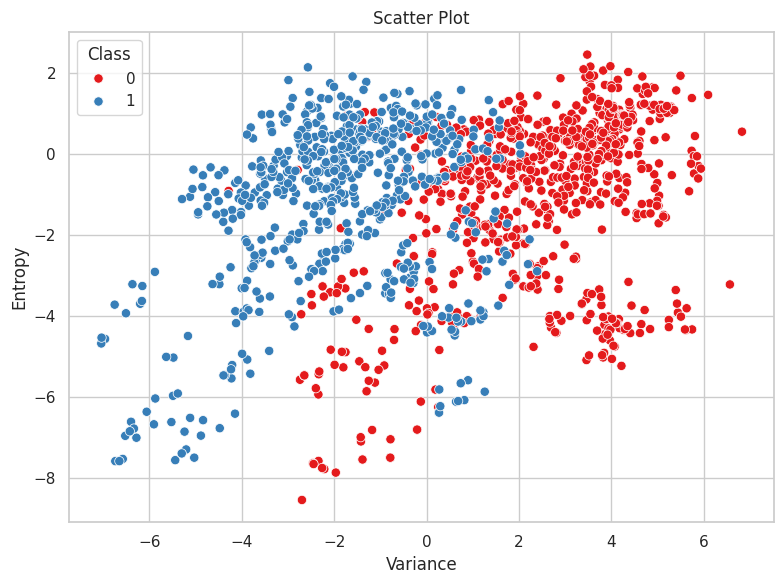
\includegraphics[width=0.66\textwidth]{scatter.png}
    \caption{Scatter Plot}
    \label{fig:scatter}
\end{figure}

The scatter plot shows that the two classes are largely separable using the selected features. This justifies the use of a Single Layer Perceptron, which performs well on linearly separable datasets.

\vspace{0.3cm}

%%%%%%%%%%%%%%%%%%%%%%%%%%%%%%%%%%%%%%%%%%%%%%%%%%%%%%%%%%%%%%

\subsection*{9.4 Box Plot}

\begin{figure}[H]
    \centering
    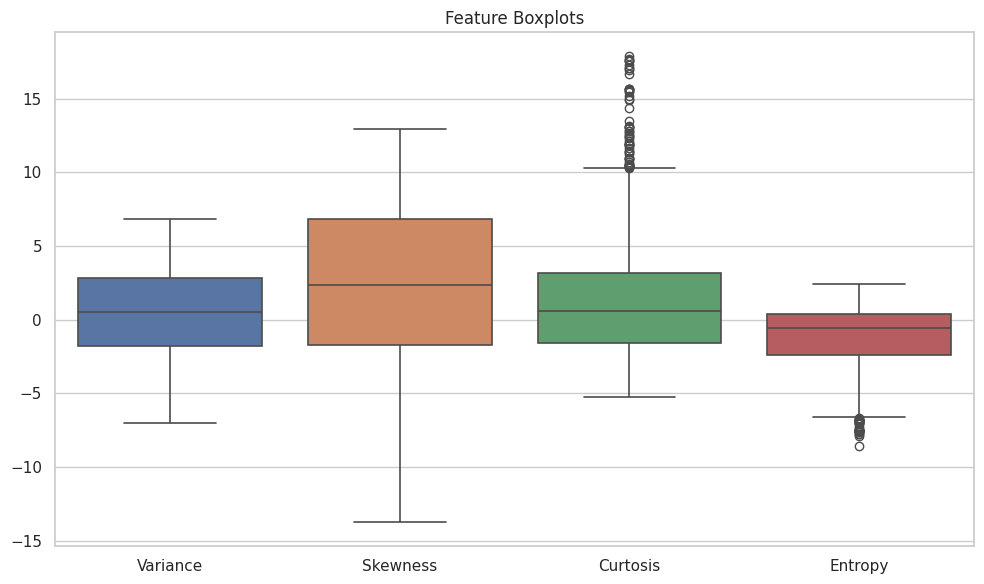
\includegraphics[width=0.66\textwidth]{box.png}
    \caption{Box Plot}
    \label{fig:box}
\end{figure}

The box plot summarizes the spread of each feature and highlights the presence of a few outliers. Since Min-Max Normalization was applied before training, these outliers did not significantly affect the learning process.

\vspace{0.3cm}

%%%%%%%%%%%%%%%%%%%%%%%%%%%%%%%%%%%%%%%%%%%%%%%%%%%%%%%%%%%%%%

\subsection*{9.5 Confusion Matrix}

\begin{figure}[H]
    \centering
    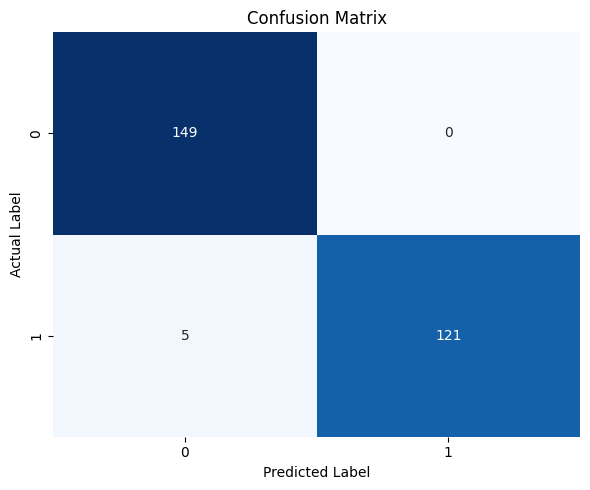
\includegraphics[width=0.63\textwidth]{confusion.png}
    \caption{Confusion Matrix}
    \label{fig:confusion}
\end{figure}

The confusion matrix indicates that the perceptron correctly classified almost every testing sample. The small number of false negatives demonstrates the effectiveness of the trained model in distinguishing authentic and forged banknotes.

\vspace{0.3cm}

%%%%%%%%%%%%%%%%%%%%%%%%%%%%%%%%%%%%%%%%%%%%%%%%%%%%%%%%%%%%%%

\subsection*{9.6 Training Error vs Epoch}

\begin{figure}[H]
    \centering
    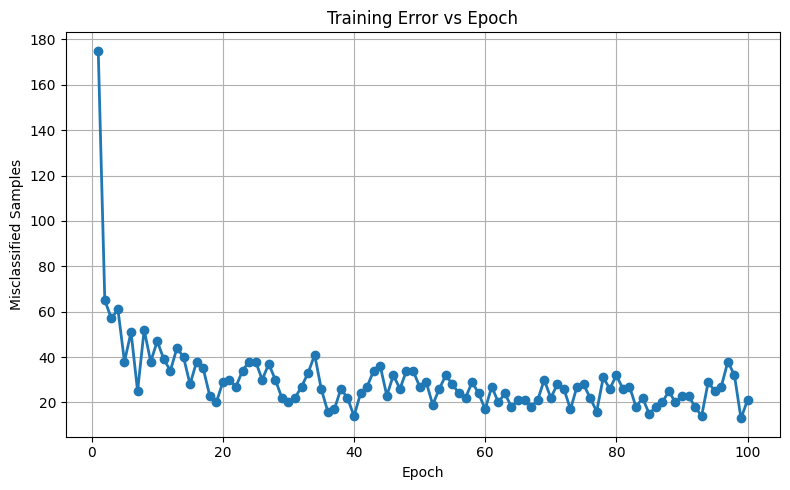
\includegraphics[width=0.58\textwidth]{error_vs_epoch.png}
    \caption{Training Error vs Epoch}
    \label{fig:error}
\end{figure}

The number of misclassified samples decreases considerably as training progresses. This behaviour indicates that the perceptron successfully learns a suitable decision boundary and gradually converges towards a stable solution.

\vspace{0.3cm}

%%%%%%%%%%%%%%%%%%%%%%%%%%%%%%%%%%%%%%%%%%%%%%%%%%%%%%%%%%%%%%

\subsection*{9.7 Weight Evolution During Training}

\begin{figure}[H]
    \centering
    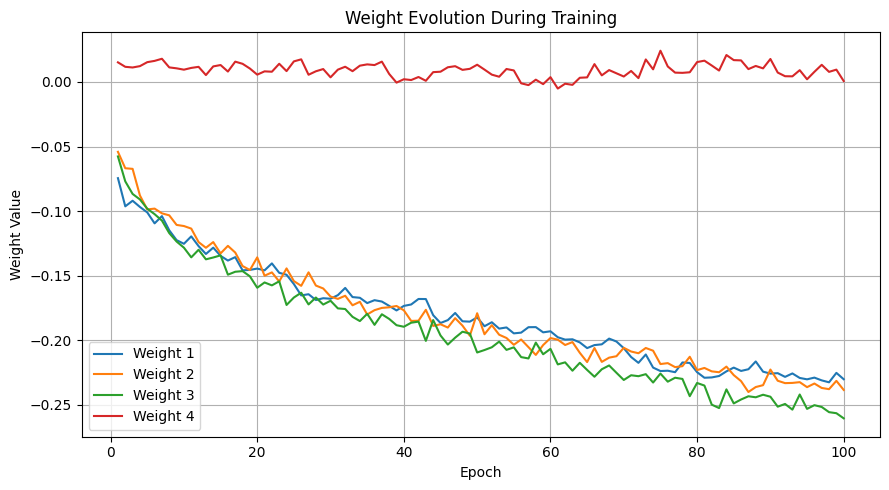
\includegraphics[width=0.72\textwidth]{weight_evaluation.png}
    \caption{Weight Evolution During Training}
    \label{fig:weights}
\end{figure}

The weight evaluation graph illustrates how the four weights are continuously adjusted during learning. Towards the final epochs the weights stabilize, indicating convergence of the learning algorithm.

\vspace{0.3cm}

%%%%%%%%%%%%%%%%%%%%%%%%%%%%%%%%%%%%%%%%%%%%%%%%%%%%%%%%%%%%%%

\subsection*{9.8 Bias Evaluation}

\begin{figure}[H]
    \centering
    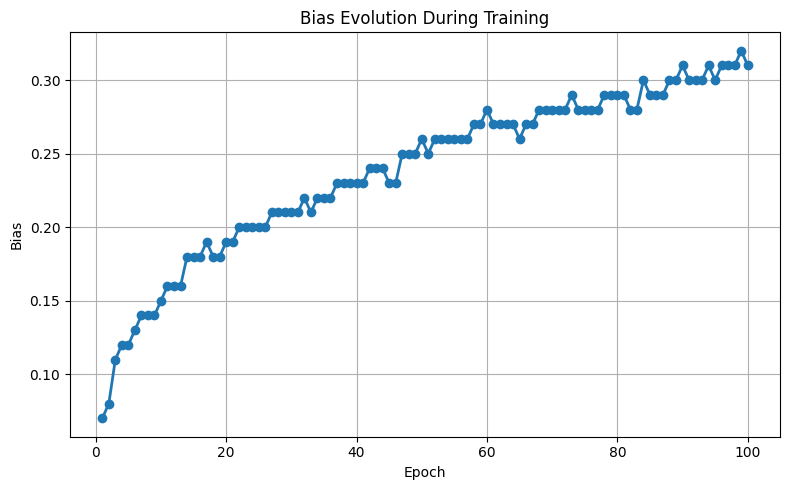
\includegraphics[width=0.68\textwidth]{bias.png}
    \caption{Bias Evaluation During Training}
    \label{fig:bias}
\end{figure}

The bias value changes gradually during training before approaching a stable value. This demonstrates that the bias contributes significantly to shifting the decision boundary and improving classification accuracy.

\vspace{0.3cm}

%%%%%%%%%%%%%%%%%%%%%%%%%%%%%%%%%%%%%%%%%%%%%%%%%%%%%%%%%%%%%%

\subsection*{9.9 Learning Rate Comparison}

\begin{figure}[H]
    \centering
    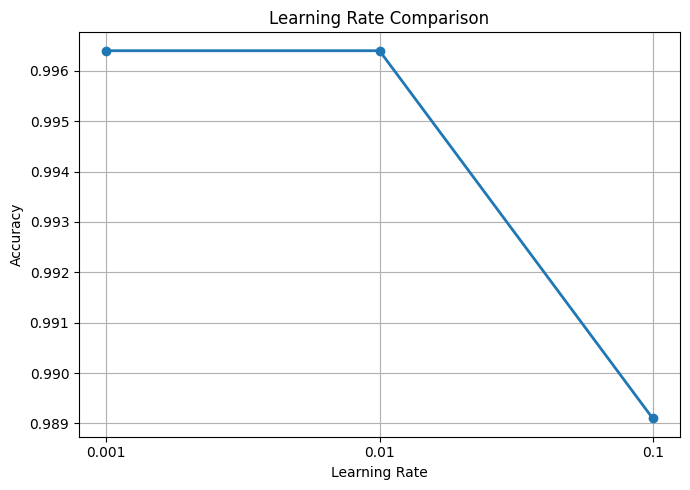
\includegraphics[width=0.68\textwidth]{lrc.png}
    \caption{Learning Rate Comparison}
    \label{fig:lrc}
\end{figure}

The comparison of different learning rates indicates that both 0.001 and 0.01 achieved the highest testing accuracy of 99.64\%. Increasing the learning rate to 0.1 resulted in a slight reduction in performance due to larger parameter updates during training.

\section*{10. Discussion}

The implementation of the Single Layer Perceptron demonstrated that a simple linear classifier can effectively solve linearly separable binary classification problems. The Banknote Authentication dataset proved to be highly suitable for perceptron learning because the two classes become nearly separable after feature normalization.

The training error decreased considerably over successive epochs, indicating that the perceptron successfully learned an appropriate decision boundary. The gradual stabilization of both the weights and bias further confirmed convergence of the learning algorithm.

The evaluation metrics indicate excellent classification performance. The model achieved an Accuracy of 98.18\%, Precision of 100.00\%, Recall of 96.03\% and an F1-Score of 97.98\%. These values demonstrate that the implemented classifier generalized well on unseen testing samples.

The learning rate experiment showed that smaller learning rates (0.001 and 0.01) produced slightly better performance than a larger learning rate (0.1). Larger learning rates resulted in comparatively larger weight updates, producing a slight reduction in testing accuracy.

Although the Single Layer Perceptron performs well on linearly separable datasets, it cannot solve non-linearly separable problems such as XOR. Such problems require multilayer neural networks together with differentiable activation functions and backpropagation learning.

%%%%%%%%%%%%%%%%%%%%%%%%%%%%%%%%%%%%%%%%%%%%%%%%%%%%%%%%%%%%%%

\section*{11. Conclusion}

In this experiment, a Single Layer Perceptron was successfully implemented from scratch using Python in Google Colab. The Banknote Authentication dataset was explored, preprocessed and normalized before training the classifier.

The perceptron learning algorithm successfully updated the weights and bias over multiple epochs, resulting in a well-trained binary classifier. The generated plots clearly illustrated the learning behaviour of the model through training error reduction, weight convergence, bias evaluation and learning-rate comparison.

The trained model achieved high classification performance with an Accuracy of 98.18\%, demonstrating that the Single Layer Perceptron is an effective solution for linearly separable binary classification tasks. The experiment also provided practical understanding of activation functions, perceptron learning, parameter updates and performance evaluation metrics.

%%%%%%%%%%%%%%%%%%%%%%%%%%%%%%%%%%%%%%%%%%%%%%%%%%%%%%%%%%%%%%

\section*{12. References}

\begin{enumerate}

\item Frank Rosenblatt,
\textit{The Perceptron: A Probabilistic Model for Information Storage and Organization in the Brain},
Psychological Review,
1958.

\item Ian Goodfellow,
Yoshua Bengio,
Aaron Courville,
\textit{Deep Learning},
MIT Press,
2016.

\item Christopher M. Bishop,
\textit{Pattern Recognition and Machine Learning},
Springer,
2006.

\item Simon Haykin,
\textit{Neural Networks and Learning Machines},
Pearson Education,
2009.

\item UCI Machine Learning Repository,
Banknote Authentication Dataset.

\url{https://archive.ics.uci.edu/dataset/267/banknote+authentication}

\item Scikit-learn Documentation.

\url{https://scikit-learn.org}

\end{enumerate}

\vfill

\end{document}